\documentclass{article}
\usepackage[utf8]{inputenc}
\usepackage[T1]{fontenc}              
\usepackage[french]{babel}
\usepackage[a4paper, margin=3cm]{geometry}
\usepackage{amsmath, amssymb, graphicx, xcolor, hyperref}


\title{Global Minimum for Active Contour Models: A Minimal Path Approach}
\author{JACOB Amaury}
\date{\today}

\begin{document}

\maketitle
\tableofcontents

\section{Introduction}
Le but de ce devoir est de comprendre, reproduire et critiquer un article.
Mon article porte sur les contours actifs par une approche du chemin minimal.
La méthode présentée dans cet article est une amélioration de la méthode des Snakes ;
cependant, cette méthode ne nécessite que deux points comme initialisation.
Elle a aussi pour avantage d'être moins sensible aux minima locaux
et de donner le chemin minimal entre les deux points.

Dans un premier temps, nous allons voir les bases mathématiques nécessaires
pour comprendre l'article.

\section{Comment calculer un contour avec un chemin minimal}
\subsection{Calcul du potentiel $P$}

Pour calculer le contour à l'aide du chemin minimal, il faut d'abord construire une 
carte de potentiel. Cette carte repose sur le gradient de l'image et sur la norme 
du gradient.

\begin{equation}
\mathbf{\nabla I} =
\begin{bmatrix}
I'_x \\[4pt]
I'_y
\end{bmatrix}
\quad\text{et}\quad
\|\nabla I\| = \sqrt{(I'_x)^2 + (I'_y)^2}.
\end{equation}

Maintenant que nous avons calculé la norme du gradient, nous pouvons déterminer le potentiel $P$.
Le potentiel $P(x,y)$ agit comme une mesure de "résistance" au passage du contour.
Ainsi, plus le gradient est fort (bord marqué), plus le potentiel est faible.
Le chemin minimal cherchera donc naturellement à suivre les bords de l'image.


Dans l'article de référence, aucune expression explicite n'est donnée pour $P$.  
J'ai donc cherché dans d'autres sources des définitions possibles du potentiel, en particulier dans deux travaux
où les formules sont simples et peu coûteuses à calculer d'un point de vue numérique :

\begin{equation}
\begin{aligned}
P_1(x,y) &= e^{-\alpha \|\nabla I(x,y)\|^2}, \\
P_2(x,y) &= \frac{1}{1 + \alpha \|\nabla I(x,y)\|^2}.
\end{aligned}
\end{equation}

Ces deux définitions apparaissent respectivement dans les articles de  
Caselles \textit{et al.}, \textit{“Geodesic Active Contours”} (1997), et  
Sethian \& Kimmel, \textit{“Computing Geodesic Paths”} (1998).

Ces deux expressions sont similaire mais une décroit de facons exponentielle 
alors que l'autre décroit en $\frac{1}{x}$ ce qui est plus lent. Le choix
dépend de l'image. 

\subsection{Calcul de la métrique $\tilde{P}$}



Une fois la carte de potentiel $P(x,y)$ calculée, elle est utilisée pour définir 
une métrique de longueur $\tilde{P}$. 
\begin{equation}
\tilde{P} = \omega + P(p)
\end{equation}
$\omega$ est un terme qui représente le lissage de la courbe et $p$ est le point 
actuel. Cette métrique joue le rôle de vitesse dans l'équation Eikonal que nous 
allons voir. 



\subsection{Equation Eikonal}



L'équation Eikonal relie $\tilde{P}(x,y)$ et une fonction de coût $U(x,y)$. Cette 
fonction représente en chaque point de l'image le coût pour aller du point de départ 
à un point $(x,y)$ de l'image.

\begin{equation}
\|\nabla U(x,y)\| = \tilde{P}(x,y),
\end{equation}
avec la condition initiale $U(p_0)=0$.

Dans l'article de Cohen et Kimmel, cette équation est résolue numériquement
par la méthode du \textit{Fast Marching}.
Cette méthode repose sur une propagation du front de niveau de $U$ :
le front avance plus rapidement dans les zones où $\tilde{P}$ est faible (autour des bords)
et plus lentement dans les zones où $\tilde{P}$ est élevée.

Mathématiquement, l'espace est discrétisé en une grille, et pour chaque pixel $(i,j)$,
on cherche la valeur de $U_{i,j}$ qui satisfait la version discrète de l'équation :
\begin{equation}
(\max\{U - U_{i-1,j}, U - U_{i+1,j}, 0\})^2 + 
(\max\{U - U_{i,j-1}, U - U_{i,j+1}, 0\})^2 = \tilde{P}_{i,j}^2.
\end{equation}
Cette équation quadratique est résolue localement à chaque itération
en utilisant uniquement les voisins déjà mis à jour.

\subsection{Back-propagation du chemin minimal}


Une fois la fonction $U(x,y)$ calculée sur toute l'image, 
on peut retrouver le contour recherché en suivant la direction opposée au gradient de $U$.
Cette étape, appelée \textit{back-propagation}, correspond à la descente du long de la pente de $U$
depuis le point d'arrivée $p_1$ jusqu'au point de départ $p_0$.
Le chemin obtenu correspond au chemin minimal reliant ces deux points 
dans la métrique $\tilde{P}$.

Mathématiquement, la courbe $C(s)$ vérifie :

\begin{equation}
\frac{dC(s)}{ds} = -\nabla U(C(s)), \quad C(0) = p_1,
\end{equation}

Quand on intègre l'expression (6) nous obtenons le chemin qui suit la pente la plus forte

Dans l'article les auteurs expliquent que cela revient à une descente de gradient
La méthode mache de facons suivante: On part de  $p_1$, et à chaque itération on choisit
le voisin possédant la plus petite valeur de $U$, jusqu'à rejoindre $p_0$.
Cette procédure simple permet de reconstruire efficacement le contour global optimal
après la propagation du front.







\section{Programmation}
\subsection{Prétraitement de l'image}

Le prétraitement est une étape clé pour obtenir des résultats cohérents.
Cette étape est la plus simple du code. Dans un premier temps, je convertis mes images en
niveaux de gris avec la fonction \texttt{open\_image}. Puis, dans un second temps, j'applique un flou 
gaussien avec un noyau de taille $5 \times 5$. Enfin, je normalise l'image en divisant
chaque pixel par 255 afin d'obtenir des valeurs de gris comprises entre $[0,1]$.


\subsection{Calcul de $\tilde{P}$}
Comme déjà vu dans la section calcul de la métrique, j'ai commencé par calculer le gradient
de l'image avec la fonction \texttt{np.gradient}, puis j'ai calculé la norme du gradient.
Pour le calcul de $P$, je peux choisir entre deux modes correspondant aux deux expressions de
$P$. Le choix du mode et des paramètres de la fonction dépend de l'image.

\subsection{Fast Marching}
Cette partie du code est la plus importante et aussi la plus longue en termes de calcul.
Le Fast Marching va permettre de déterminer $U$ (la carte de distance).

\subsubsection{Initialisation}
La carte de distance est de même dimension que l'image et, au départ, toutes les valeurs de
$U$ sont initialisées à l'infini, sauf le point de départ qui est initialisé à 0. 
Au même moment, j'initialise un autre tableau de même dimension que l'image nommé 
\texttt{labels}. \texttt{Labels} est constitué de trois valeurs décrites dans 
l'article : \textit{Far}, \textit{Trial} et \textit{Alive}. Toutes les valeurs de 
\texttt{labels} sont initialisées à \textit{Far}, sauf le point $p_0$ qui est à 
\textit{Trial}. Il ne reste que la liste des points à traiter (\texttt{heaps}), 
initialisée avec le tuple des coordonnées de $p_0$. Dans l'article, les auteurs 
précisent qu'il est préférable d'utiliser une structure de type \textit{min-heap}. 
En Python, il existe le module \texttt{heapq} pour cela, mais n'étant pas familier 
avec cette syntaxe, je n'ai pas réussi à faire une version de mon code opérationnelle avec.

\subsubsection{Boucle principale}
On va itérer jusqu'à ce que \texttt{heap} soit vide. À chaque itération, on va 
trouver la valeur de distance minimale ($\min(U)$) des points stockés dans 
\texttt{heap} et sauvegarder les coordonnées et la distance minimale. Puis nous 
retirons les coordonnées de ce pixel de \texttt{heap}, et le label de ce pixel 
passe à \textit{Alive}.

Finalement, je regarde les voisins de ce pixel avec une connexité de 4. 
Si ces pixels ne sont pas à \textit{Alive}, je calcule leur nouvelle distance à l'aide de la fonction 
\texttt{solve\_eikonal} (qui sera détaillée dans la section suivante). 
Si cette distance est inférieure à la distance de la carte de distance, elle devient la nouvelle distance, 
et si le label de ce pixel est à \textit{Far}, je l'ajoute à \texttt{heap} et son label passe à \textit{Trial}.


\subsubsection{Solve eikonal}

Dans un premier temps, je récupère la valeur de $\tilde{P}$ au pixel courant.  
Ensuite, je regarde les voisins gauche et droite pour calculer la plus petite 
distance $a$, et les voisins haut et bas pour la plus petite distance $b$.  
Ces valeurs $a$ et $b$ représentent la distance minimale connue autour du pixel 
dans les deux directions.  

Ensuite, je vérifie la différence entre $a$ et $b$.  
Si le front arrive des deux directions, je résous l'équation quadratique issue 
de la discrétisation de l'équation d'Eikonal :  
\[
U_{new} = \frac{a + b + \sqrt{2 \tilde{P}^2 - (a - b)^2}}{2}.
\]
Enfin, la fonction retourne cette nouvelle valeur $U\_{new}$, 

\subsection{Fonction \texttt{backtrack}}

Cette fonction permet de retrouver le chemin minimal une fois la carte de distance 
$U$ calculée. Pour cela, je calcule le gradient local de $U$ autour du point courant, 
puis je me déplace dans la direction opposée au gradient normalisé.  
Le pas de déplacement est défini par la variable \texttt{step}.  
À chaque itération, je sauvegarde les nouvelles coordonnées dans la liste 
\texttt{paths}. Cette boucle se répète jusqu'à atteindre le point de départ 
ou jusqu'à atteindre le nombre maximal d'itérations \texttt{max\_it}.  
Le résultat est donc une suite de points représentant le chemin minimal entre les 
deux points.






\section{Résultats}

\subsection{Image similaire à l'article}


Dans cette partie, nous allons voir les résultats de l'implémentation de la méthode
vue dans l'article.

J'ai décidé, pour les tests, de commencer sur des images très proches de celles
montrées dans l'article. Nous avons donc choisi des images de chemins vues du ciel,
présentant un contraste fort entre le chemin et le reste de l'image.

\begin{figure}[h!]
    \centering
    \begin{minipage}{0.24\textwidth}
        \centering
        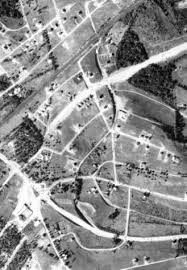
\includegraphics[width=\linewidth]{result_image/Image_2/1.jpg}
        \caption*{\small Image de base}
    \end{minipage}\hfill
    \begin{minipage}{0.24\textwidth}
        \centering
        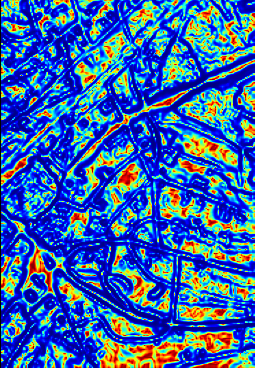
\includegraphics[width=\linewidth]{result_image/Image_2/2.png}
        \caption*{\small Carte des $\tilde{P}$}
    \end{minipage}\hfill
    \begin{minipage}{0.24\textwidth}
        \centering
        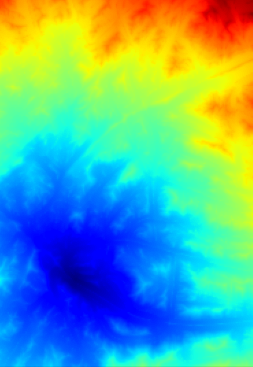
\includegraphics[width=\linewidth]{result_image/Image_2/3.png}
        \caption*{\small Carte des distances}
    \end{minipage}\hfill
    \begin{minipage}{0.24\textwidth}
        \centering
        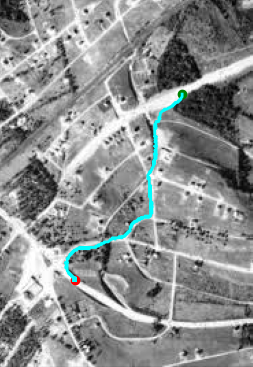
\includegraphics[width=\linewidth]{result_image/Image_2/4.png}
        \caption*{\small Image de base et chemin}
    \end{minipage}
    \label{fig:images-tests}
\end{figure}

La figure 1 est l'image utilisée dans cet exemple. Elle est similaire à l'image présentée 
dans l'article.

La figure 2 représente la carte de $\tilde{P}$. On peut voir que les bords des chemins 
sont en bleu très sombre, ce qui signifie que le coût local est faible à ces endroits. 
Le front se propage donc plus rapidement le long des contours. 
On remarque aussi que l'intérieur des chemins est en rouge, ce qui indique un coût 
plus élevé et donc une propagation plus lente dans ces zones homogènes.

La figure 3 représente la carte des distances $U$. Comme nous pouvons le voir, plus 
on s'éloigne du point de départ au centre de l'image, plus les couleurs deviennent 
rouges, ce qui correspond à une distance cumulée plus grande. On observe également que 
là où se trouvent les chemins, les distances sont plus faibles, car le coût local y 
est minimal.

La figure 4 représente le chemin trouvé à l'aide du backtracking. 
Les résultats sur cette image sont très satisfaisants : le chemin suit bien le tracé 
du chemin réel visible sur l'image et reste stable malgré les petites variations de contraste.



\subsection{Image différente de l'article}


Dans cette section nous allons voir les résultats de la méthode dans le cadre d'une
image plus réaliste et avec un contraste moins marqué entre la route et le bord de 
la route.


\begin{figure}[h!]
    \centering
    \begin{minipage}{0.24\textwidth}
        \centering
        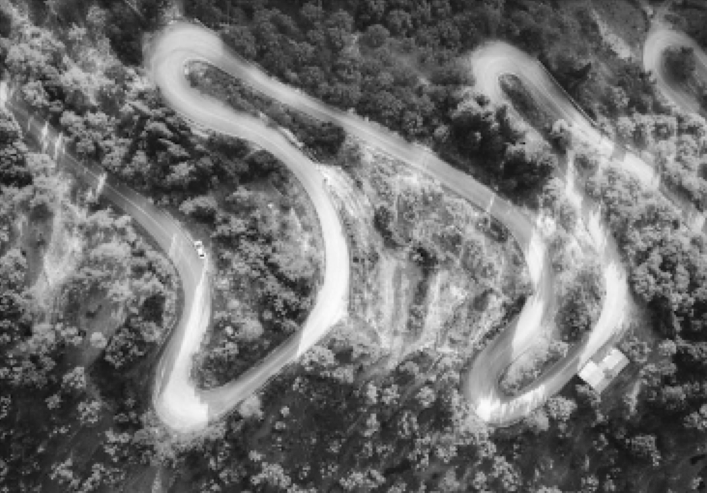
\includegraphics[width=\linewidth]{result_image/Image_4/1.png}
        \caption*{\small Image de base}
    \end{minipage}\hfill
    \begin{minipage}{0.24\textwidth}
        \centering
        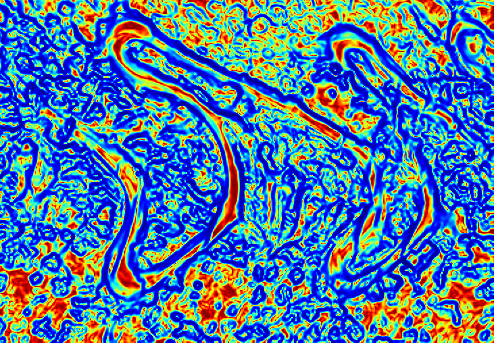
\includegraphics[width=\linewidth]{result_image/Image_4/2.png}
        \caption*{\small Carte des $\tilde{P}$}
    \end{minipage}\hfill
    \begin{minipage}{0.24\textwidth}
        \centering
        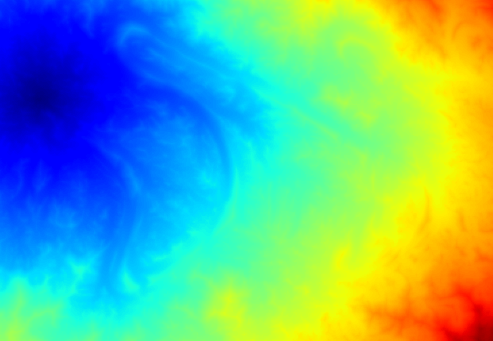
\includegraphics[width=\linewidth]{result_image/Image_4/3.png}
        \caption*{\small Carte des distances}
    \end{minipage}\hfill
    \begin{minipage}{0.24\textwidth}
        \centering
        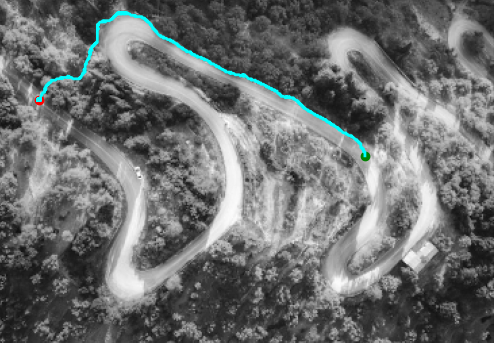
\includegraphics[width=\linewidth]{result_image/Image_4/4.png}
        \caption*{\small Image de base et chemin}
    \end{minipage}
    \label{fig:images-tests}
\end{figure}

Comme nous pouvons le voir, l'algorithme a du mal à distinguer la route du reste de la forêt. 
La figure 6 montre la carte de $\tilde{P}$, où le contraste entre la route et l'environnement 
est faible. La figure 7 présente la carte des distances $U$, qui reste donc assez uniforme 
et ne met pas clairement en évidence le tracé du chemin.



\section{Conclusion}

Comme nous avons pu le voir, l'implémentation de la méthode offre des résultats
satisfaisants sur les images ayant un fort contraste entre le chemin et le bord
du chemin. Cependant, dès que l'image ne présente pas un fort contraste, la méthode
devient inefficace.

Les temps de calcul observés sont vraiment moins bons que ceux énoncés dans l'article.
Cela est sûrement dû au fait que je n'utilise pas \texttt{heapq}, mais surtout au fait que Python
n'est pas un langage aussi puissant que le C ou le C++, qui sont compilés et permettent 
de faire des calculs sur plusieurs cœurs et threads. Cela est aussi sûrement dû 
à mon inexpérience dans le domaine.

Il existe plusieurs méthodes plus modernes qui pourraient remplacer cette méthode,
comme par exemple un réseau de neurones de type \textit{CNN} pour la détection automatique des bords.
Cette approche aurait sûrement de meilleurs résultats, mais surtout serait plus rapide grâce
aux calculs effectués sur GPU.

Pour conclure, ce travail était vraiment intéressant, tant sur le plan de la compréhension
de l'article que sur celui de la programmation.




\end{document}
